\chapter{Methodology}
\label{chap:lr}
\chaptermark{Second Chapter Heading}

% ____________ include an overview of methodology ___________
In this chapter we will discuss the control strategy of a TSA driven setup consisting of a single string. To design all considered methods of force estimation (based on the increases of the motor current, Classic momentum observer and Sliding Mode momentum observer) a mathematical model of the TSA is required, which is discussed in Section I. Using the configuration of the TSA and proprioceptive measures (motor angular displacement $\theta$, string's linear displacement $X$ and their respective velocities $\dot \theta, \dot X$ or both options whenever convenient), we can find the system's Jacobian $\mathbb{J}$, dynamics, the total energy $E$ of TSA and its Lagrangian $L$. The Jacobian and the dynamics of the system are needed for all considered methods  The Lagrangian is used to obtain the time differential of the generalized momentum $\dot p$, which is a key component in the Classical Momentum Observer and Sliding Mode Momentum Observers. 

The design of classical momentum observer is presented in Section II, where the general strategy of obtaining the momentum's residual and using it to estimate external torque is discussed \cite{coll_avoid}. After which, the external force can be found using the obtained torque and the Jacobian of the system.

Based on the classical variant, in Section III a Sliding Mode Disturbance Observer is designed to improve the force control model by disposing of a phase lag in the estimated external torque signal caused by the momentum observer's first-order characteristic \cite{sliding_mode}.


\section{Mathematical Model of TSA}

Before we touch on the subject of force estimation and momentum observers, it is vital to overview the mathematical model of the TSA used in the experimental setup. A more detailed model that considers all other TSA features is described in works \cite{TSA_intro}, \cite{TSA_oscillations}, \cite{TSA_math_model}.


\subsection{Kinematics}
    In accordance with the approximate image of the section of the twisted string shown in Fig.1(a), the cable with length $L$, radius $r$ twisted by angle $\theta$ forms a spiral and contracts linearly by $X$.
    This section unwraps into a right-angled triangle with sides $(L-X)$, $L$ and $\theta r$, where: 
    \begin{equation}
        L^2 = (L-X)^2 + \theta^2r^2
    \end{equation}
    Note here that equation above is a second order polynomial, therefore there exist two solutions for motor angle $\theta$ that correspond to the same string contraction level $X$.

    The differentiation of the constraint above with respect to time yields the relationship between the payload (output) and motor (input) velocities:
    \begin{equation}
        \dot X = \mathbb{J}(\theta, X) \dot \theta
    \end{equation}
    where $\mathbb{J}$ is the Jacobian of twisted strings:
    \begin{equation}
        \mathbb{J} = \frac{\theta r^2}{L-X} = \frac{\theta r^2}{\sqrt{L^2 - \theta^2 r^2}} = \frac{r\sqrt{L^2 - (L-X)^2}}{L-X}
    \end{equation}

    \begin{figure}
        \centering
        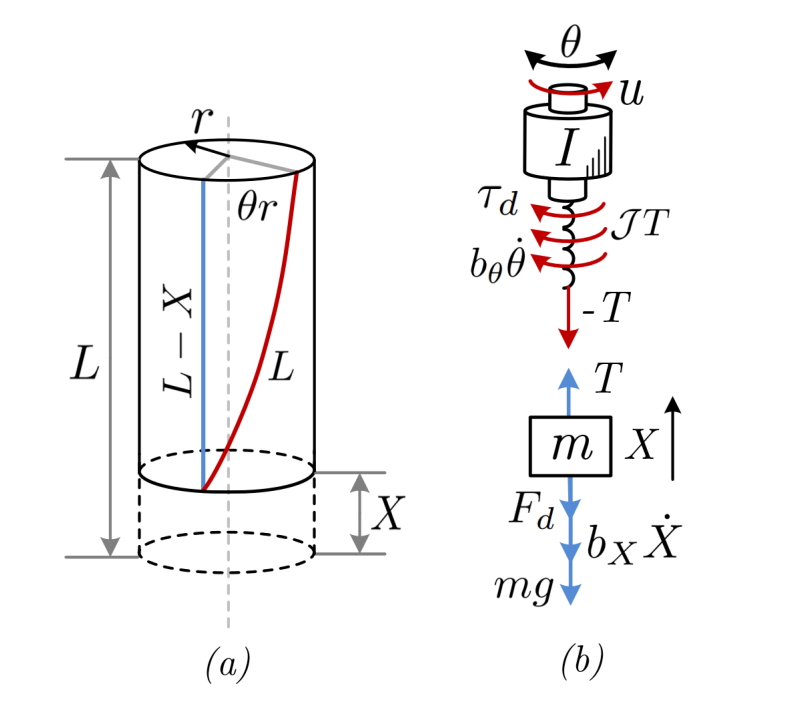
\includegraphics[width=0.6\linewidth]{figs/schematic_model.png}
        \caption{Schematic diagrams for the analysis of TSA kinematics (a) and dynamics (b)}
        \label{fig:tsa_diagram}
    \end{figure}


\subsection{Energy}

The energy of the TSA can be represented with respect to the motor angle $\theta$, string's linear contraction $X$ or both, depending on the availability and convenience of motor and payload variables. Total energy of TSA is the sum of the system's kinetic, potential and dissipated energies:
\begin{equation}
    E = E_K + E_P + E_D = \frac{1}{2}I\dot\theta^2 + (\frac{1}{2}m\dot X^2 + mgX) + E_D
\end{equation}
where $I$ is the motor's inertia and $g$ is the gravitational constant. 
Using the kinetic $E_K$ and potential $E_P$ energies a Lagrangian $L$ can be derived as:
\begin{equation}
    L = E_K - E_P = \frac{1}{2}I\dot \theta^2 - \frac{1}{2}m\dot{X}^2 - mgX
\end{equation}


\subsection{Dynamics}
The robot dynamics can be defined using a Lagrangian approach:
\begin{equation}
    M(q)\ddot q + C(q,\dot q)\dot q + g(q) = \tau_m + \tau_{ext}
\end{equation}
where $q$ is the set of generalized coordinates; $M(q)>0$ is the symmetric positive definite inertia matrix;  $g(q)$ is the gravity vector; $\tau_m$ is the motor torque; $\tau_{ext}$ is the external torque$C(q,\dot q)$ is the Coriolis matrix satisfying the passivity property:
\begin{equation}
    \dot M(q) = C(q,\dot q) +  C(q,\dot q)^T 
\end{equation}

The Equations of Motion (EoM) can be derived using the Euler-Lagrange approach of TSA as follows:
\begin{equation}
    \begin{cases}
        \tau_m = I\ddot \theta + \mathbb{J}T + b_{\theta}\dot \theta + \tau_{ext} \\
        T = m\ddot X +mg+ b_X\dot X + F_{ext}
    \end{cases}
\end{equation}
where  $T$ - string's tension; $b_{\theta}, b_X$ - viscous friction coefficients in motor and payload, respectively; $\tau_{ext}$ and $F_{ext}$ - external disturbances.

Notice, that since the considered robotic system is a 1-DOF (degree of freedom) system with one string, external forces can be derived from external torques using the system's Jacobian:
\begin{equation}
    \tau_{ext} = \mathbb{J}F_{ext}
\end{equation}

The EoM can be rewritten with respect to motor angle as follows:
\begin{equation}
    \begin{cases}
        \tau_m = M_{\theta} \ddot\theta + h_{\theta}(q,\dot q)\\
        M_{\theta} = I + m\mathbb{J}^2\\
        h_{\theta} = (b_{\theta}+\mathbb{J}(m \dot{\mathbb{J}} + b_X))\dot\theta + \mathbb{J} (mg + F_{ext})+\tau_{ext}
        
    \end{cases}
\end{equation}

Similarly, we rewrite the dynamics with respect to payload as follows:
\begin{equation}
    \begin{cases}
        \tau_m = M_{X} \ddot X + h_{X}(q,\dot q)\\
        M_{X} = I + m\mathbb{J}^{-2}+m\\
        h_{X} = (\math{J}^{-1}b_{\theta}+\mathbb{J}^{-2} \dot{\mathbb{J}}I+ b_X)\dot X + \mathbb{J} (mg + F_{ext})+\tau_{ext}
        
    \end{cases}
\end{equation}


\section{Classical Momentum Observer}

    The derivation of all momentum observers is based on the timely evolution of the generalized momentum of the robot \cite{collision}. Since momentum $p$ is the derivative of the Lagrangian $L$ with respect to generalized velocities $\dot q$, using Euler-Lagrange Equation, we can express the time derivative of the momentum $\dot p$:
\begin{equation}
    \frac{d}{dt}(\frac{\delta L}{\delta \dot q}) - \frac{\delta L}{\delta q} = \tau_{ext}
\end{equation}
    

\begin{equation} 
    \dot p = \frac{\delta L}{\delta q} + \mathbb{J}F_{ext}
\end{equation}
where the par
$$
    \frac{\delta L}{\delta q} = I\dot{\theta}\ddot{\theta} - m\dot{X}\ddot{X} - mg\dot X
$$

    The derivation of the classic first-order momentum observer is based on the residual
\begin{equation}
    \textbf{r} = K_O( p - \int_0^t{(\frac{\delta L}{\delta q} + r)}ds - p_0 )
\end{equation}
    where $p_0$ is the initial value of the generalized momentum and $K_O = diag(k_O, i)>0$.

    By using the acquired $\dot p$, the time derivative of the residual is:
\begin{equation}
    \dot r = -K_O(r - \tau_{ext})
\end{equation}
This means that residual $r$ is a first-order filtered version of $\tau_{ext}$ and therefore it can be used as an estimation of the external torques and subsequently external forces using (3.9).